
\documentclass{article}
    \usepackage[utf8]{inputenc}
    \usepackage[T2A]{fontenc}
    \usepackage[english,russian]{babel}

    % Related to math
    \usepackage{amsmath,amssymb,amsfonts,amsthm}

    \usepackage{graphicx}
    \usepackage{subfigure}
    \graphicspath{{media/}}

    \usepackage{multirow}

\begin{document}

\section{Практические аспекты оптимизации траектории инструмента для машин лазерной резки с ЧПУ}

\subsection{Точное вычисление целевых функций в задаче оптимизации маршрута резки на примере машины лазерной резки ByStar3015}

Как мы отмечали в Параграфе 1.2
%%% TODO fix reference  ^^^^^^^^^^^^^^^
для задачи оптимизации маршрута резки (\ref{problem-statement})
проблема точного вычисления целевых функций времени резки и стоимости резки,
определяемых, в частности, формулами (\ref{cutting-time}) и (\ref{cutting-cost}):
$$
T_{cut} = \frac{L_{on}}{V_{on}} + \frac{L_{off}}{V_{off}} +N_{pt} \cdot t_{pt}
$$
$$
F_{cost}=
L_{on} \cdot C_{on} +
L_{off} \cdot C_{off} +
N_{pt} \cdot C_{pt}
$$
является малоисследованной.
Ниже будут приведены результаты исследований,
проведенных А.Ф.Таваевой на предприятии
АО «Производственное объединение “Уральский оптико – механический завод”
имени Э.С. Яламова» (Екатеринбург)
на машине лазерной резки ByStar3015.
Более подробно результаты этих исследований изложены в
\cite{intro45,intro46,intro47}.

\subsubsection{Вычисление фактического времени лазерной резки машины с ЧПУ
в зависимости от параметров управляющей программы и технологических факторов процесса резки}

Неточность вычисления фактического времени резки
$T_{cut}$
связана с тем, что скорость рабочего хода машины с ЧПУ
$V_{on}$,
программируемая в управляющей программе как константа,
фактически таковой не является и может меняться
в зависимости от различных технологических факторов,
а также характеристик спроектированной управляющей программы.
В частности, было установлено,
что при увеличении числа кадров в управляющих программах
резки разных наборов заготовок,
имеющих один и тот же суммарный периметр контуров,
фактическая средняя скорость резки падает.
Причины, по которым УП могут содержать большое количество кадров,
в основном, связано с тем, что контуры со сложной геометрией
(например, сплайны) при конвертации из CAD системы в CAM
модуль из-за разницы в геометрических форматах файлов
разбиваются на большое число геометрических примитивов
(например, на отрезки прямых и дуги окружностей),
т.е. аппроксимируются более простыми геометрическими примитивами.
Разница в форматах, в свою очередь,
вызвана тем, что практически все системы ЧПУ
оснащаются только линейными и круговыми интерполяторами.
Как правило, аппроксимация сложной геометрии сводится
именно к линейной аппроксимации.
Иногда конвертеры CAD файлов аппроксимируют отрезками прямых
даже дуги окружностей, хотя в этом нет необходимости,
если система ЧПУ поддерживает круговую интерполяцию.

Ниже приведены некоторые практические результаты
по определению зависимости скорости рабочего хода
инструмента лазерного комплекса ByStar3015
от количества кадров управляющей программы.

Исследования были проведены для следующих материалов:
10кп ($\Delta$=1-10мм) и АМг3М ($\Delta$=1-5мм).
Для проведения вычислительных экспериментов были разработаны
150 тестовых УП для резки различных фигурных заготовок с числом кадров
$n=\overline{10,5000}$
для материала 10кп и 150 УП – для материала АМг3М с числом кадров
$n=\overline{10,2000}$.

Статистический материал был обработан в программе “Mathcad”
и с помощью метода наименьших квадратов были построены
аппроксимирующие функции для зависимости скорости
рабочего хода инструмента
$V_{on}$
от количества кадров в спроектированной УП.
По результатам эксперимента были сделаны следующие выводы:

\begin{enumerate}
\item Фактическая средняя скорость рабочего хода режущего инструмента
$V_{on}$
является монотонно убывающей функцией от числа кадров УП
(рис. \ref{amg3m}, \ref{10kp});

\item Заданная в УП скорость
$V_{on}$
совпадает с фактической средней скоростью
при достижении числа кадров некоторого порогового значения $N$.
Когда количество кадров в УП меньше порогового значения $n<N$,
то фактическая скорость выше заданной,
а при увеличении числа кадров больше порогового $n>N$
– может существенно снижаться
(в проведенных экспериментах снижение средней
фактической скорости режущего инструмента по сравнению
с заданным в УП значением доходило до 70\%);

\item Пороговое значение различно для разных марок материала и толщин.

\end{enumerate}

Для изложения результатов вычислительных экспериментов
введём следующие обозначения:
пусть
$n$  – число кадров в УП,
$V_\text{факт}$  – фактическая средняя скорость режущего инструмента при заданной скорости $V_{on}$,
$N$ - число кадров (пороговое значение), для которого $V_\text{факт}=V_{on}$;
$\sum \varepsilon_n^2$  - сумма квадратов отклонений исходных значений
скорости режущего инструмента и значений аппроксимирующей функции $V_{on}(n)$
в этих точках.

При аппроксимации точечных графиков
зависимости фактической скорости
$V_\text{факт}$
от числа кадров $n$
в УП аппроксимирующими кривыми в “Mathcad”
для всех значений исследуемых марок материала и толщин материала было установлено,
что значения
$\sum \varepsilon_n^2 \to 0$
достигаются при аппроксимации экспериментальных данных логарифмической функцией.

Аналогичные результаты были получены для материала АМг3М $\Delta$=2-5мм и 10кп $\Delta$=1-10мм.
Обобщенные результаты для всех исследованных марок материала и толщин приведены в табл. \ref{v-formulae}.

При использовании материала других марок
необходимо проведение дополнительных исследований,
либо использование имеющихся данных по материалу
с близкими физическими свойствами.

\begin{figure}
  \begin{center}
  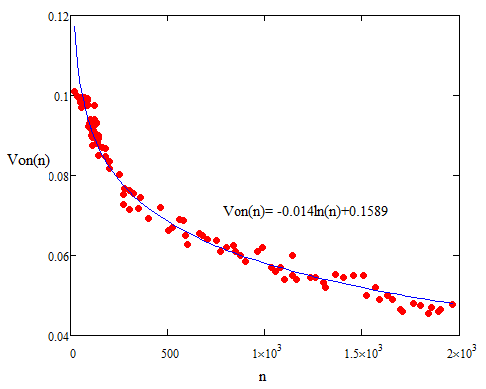
\includegraphics[width=0.7\textwidth]{amg3m.png}
  \caption{Изменение скорости режущего инструмента на рабочем ходе для АМг3М, $\Delta$=1мм ($n=\overline{10,2000}$)}
  \label{amg3m}
  \end{center}
\end{figure}


\begin{figure}
  \begin{center}
  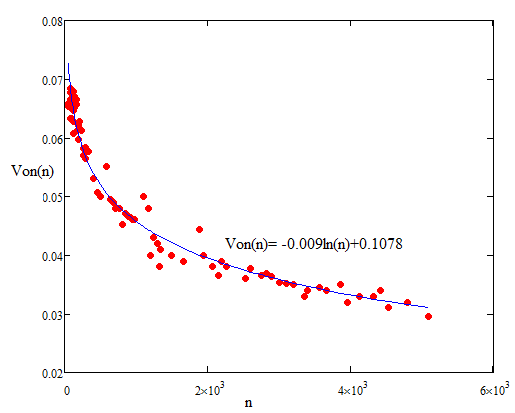
\includegraphics[width=0.7\textwidth]{10kp.png}
  \caption{Изменение скорости режущего инструмента на рабочем ходе для 10кп, $\Delta$=3мм ($n=\overline{10,5000}$)}
  \label{10kp}
  \end{center}
\end{figure}

\begin{table}
  \begin{tabular}{lll}
    Материал & Толщина, мм & Формула расчёта $V_{on}$ \\
    \hline
    \multicolumn{3}{c}{$n=\overline{10,5000}$} \\
    10кп & 1 & $V_{on} = -0.024 \ln n+0.245$ \\
    10кп & 2 & $V_{on} = -0.015 \ln n+0.1686$ \\
    10кп & 3 & $V_{on} = -0.009 \ln n+0.1078$ \\
    10кп & 3.5 & $V_{on} = -0.006 \ln n+0.0756$ \\
    10кп & 4 & $V_{on} = -0.006 \ln n+0.0709$ \\
    10кп & 8 & $V_{on} = -0.003 \ln n+0.0442$ \\
    10кп & 10 & $V_{on} = -0.002 \ln n+0.0365$ \\
    \multicolumn{3}{c}{$n=\overline{10,2000}$} \\
    АМг3М & 1 & $V_{on} = -0.014 \ln n+0.1589$ \\
    АМг3М & 1.5 & $V_{on} = -0.001 \ln n+0.011$ \\
    АМг3М & 3 & $V_{on} = -0.004 \ln n+0.0672$ \\
    АМг3М & 4 & $V_{on} = -0.001 \ln n+0.0301$ \\
    АМг3М & 5 & $V_{on} = -6\cdot 10^{-4} \ln n+0.0177$ \\
  \end{tabular}
  \label{v-formulae}
  \caption{Обобщенная таблица формул для вычисления рабочей скорости инструмента на лазерном комплексе ByStar3015}
\end{table}

Рассмотрим пример оптимизации времени резки
$T_{cut}$
(\ref{cutting-time})
при резке 15 фигурных заготовок для задачи
(материал АМг3М $\Delta$=1мм).
Раскройная карта (рис. \ref{amg-cutting})
содержит 15 заготовки двух типоразмеров,
при этом количество граничных контуров заготовок равно 19.
Каждый контур вырезается с помощью резки
«по замкнутому контуру».
С целью сокращения множества допустимых решений
задачи множество возможных точек врезки было
ограничено конечным множеством (задача GTSP),
состоящим из 55 точек
(обозначены квадратами зеленого цвета;
соответствующие точки выключения инструмента обозначены крестиками).
Для решения задачи использован точный алгоритм ДП.
УП резки для данного примера содержат 120 команд или кадров
(т.е. $n=120$),
которые включают команды перемещения инструмента
для резки контуров
(с учетом разбиения каждого контура на несколько геометрических примитивов)
на рабочем ходе,
команды перемещения инструмента на холостом ходе
и ряд технологических команд.
Скорость рабочего хода инструмента, заданная в УП,
$V_{on}=0.1$ м/с.

\begin{figure}
  \begin{center}
  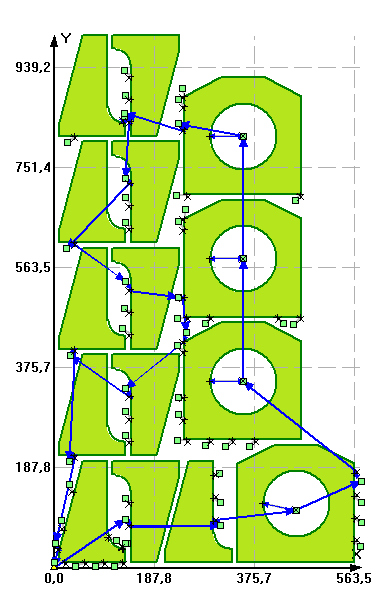
\includegraphics[width=0.5\textwidth]{amg-cutting.png}
  \caption{Раскройная карта и оптимальный по времени маршрут
  перемещения режущего инструмента для 15 заготовок (материал АМг3М $\Delta$=1мм) при условии, что
  $V_{on}=const=0.1$м/с}
  \label{amg-cutting}
  \end{center}
\end{figure}

На рис. \ref{amg-cutting}
показан маршрут резки
(перемещение инструмента на холостом ходе показаны стрелками синего цвета),
для которого значение целевой функции
$T_{cut}$ (\ref{cutting-time})
при
$V_{on}=0.1$ м/с
составляет
$T_{cut}=126.27$ сек.
Однако фактическое время резки по управляющей программе,
составленной для этого маршрута, оказалось (как и ожидалось)
значительно больше,
поскольку число кадров в программе ($n=120$)
значительно больше порогового значения $N=70$
для материала АМг3М $\Delta$=1мм.

При использовании значения
$V_{on}=-0.014 \ln n + 0.1589$
(табл.6) в целевой функции (\ref{cutting-time})
оптимизационная процедура ДП
даёт другое оптимальное решение задачи,
которое показано на рис. \ref{amg-optimal}.
Тогда среднее фактическое значение рабочей скорости инструмента при $n=120$
составило
$V_{on}=0.0919$ м/с.
В свою очередь для оптимального маршрута резки значение времени резки составило
$T_{cut}=141.38$ сек.

Таким образом,
точное вычисление целевой функции для
данного примера обеспечило не только
точное вычисления значения экстремума
целевой функции, но и другой (правильный)
результат поиска оптимального маршрута резки,
полученный  с учетом числа кадров УП.


\begin{figure}
  \begin{center}
  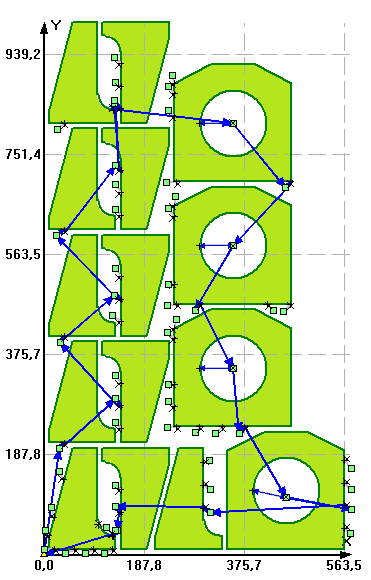
\includegraphics[width=0.5\textwidth]{amg-optimal.png}
  \caption{Оптимальный по времени маршрут перемещения режущего инструмента при условии, что
  $V_{on}=-0.014 \ln n + 0.1589$
  $(n=120)$}
  \label{amg-optimal}
  \end{center}
\end{figure}

Данный пример иллюстрирует необходимость
получения табли+ц типа Таблицы \ref{v-formulae}
при решении конкретных оптимизационных задач
маршрутизации инструмента машин листовой резки с ЧПУ.

\subsubsection{Вычисление стоимости резки заготовок на машине машине с ЧПУ в режиме моделирования процесса резки}

Другая проблема точного вычисления целевой функции
при оптимизации маршрута резки связано
с поиском адекватных значений стоимости в формуле (\ref{cutting-cost})
$$
F_{cost}=
L_{on} \cdot C_{on} +
L_{off} \cdot C_{off} +
N_{pt} \cdot C_{pt}
$$

Напомним:
$C_{on}$ – стоимость единицы пути с включенным режущим инструментом;
$C_{off}$ – стоимость единицы пути с выключенным режущим инструментом;
$C_{pt}$ – стоимость одной точки врезки,
$L_{off}$ – длина переходов с выключенным режущим инструментом (холостой ход);
$L_{on}$ – длина реза с включенным режущим инструментом;
$N_{pt}$ – количество точек врезки.

Рассмотрим вопрос точного вычисления
стоимости лазерной резки в задаче
оптимизации маршрута режущего инструмента
применительно к машине лазерной резки (тип лазера: СО$_2$)
с ЧПУ на примере машины ByStar3015.

Проблема точного вычисления целевой функции
при оптимизации маршрута резки связана с
поиском адекватных значений стоимости
$F_{cost}$,
вычисление которой зависит от параметров
$C_{on}, C_{off}, C_{pt}$.

Для расчета
$C_{on}$
введем следующие обозначения для стоимостных параметров,
вычисляемых на 1 м рабочего хода инструмента:
$C_\text{расх}$   - стоимость расходных материалов (например, сопло, защитное стекло, газовые трубки);
$C_\text{тех}$   - стоимость технологического газа (азот или кислород в зависимости от типа обрабатываемого материала);
$C_\text{лаз}$ - стоимость лазерного газа (при работе на машине с ЧПУ на проточном газовом лазере),
$C_\text{э/э}^{on}$ - стоимость электроэнергии;
$C_\text{зп}^{on}$ - затраты, связанные с заработной платой сопровождающего персонала;
$C_\text{А}^{on}$ - амортизация оборудования.
Тогда в общем виде
$C_{on}$
будем вычислять по следующей формуле:

\begin{equation}
  C_{on} =
  C_\text{э/э}^{on} +
  C_\text{тех} +
  C_\text{лаз} +
  C_\text{расх} +
  C_\text{зп}^{on} +
  C_\text{А}^{on}
  \label{c-on}
\end{equation}

Для вычисления значений
$C_{on}, C_\text{э/э}^{on}, C_\text{тех}, C_\text{лаз}, C_\text{расх}, C_\text{зп}^{on}, C_\text{А}^{on}$
введем дополнительные обозначения:
$t_{on}$ – время, затрачиваемое на один метр рабочего хода инструмента, час;
$P_{on}$ – затраты электроэнергии за один час работы лазерного комплекса на рабочем ходе, кВт/ч;
$V_\text{тех}$ – расход технологического газа, м$^3$/ч;
$V_\text{лаз}$ – расход лазерного газа, м$^3$/ч;
$C_\text{э/э}$ - стоимость электроэнергии за 1 кВт;
$C_{\text{лазМ}^3}$- стоимость 1м$^3$ лазерного газа;
$C_{\text{техМ}^3}$ - стоимость 1м$^3$ технологического газа;
$C_\text{расхЕд}$- стоимость единицы расходных материалов;
$t_\text{расхСрок}$- срок службы расходных материалов;
$C_\text{зп}$ - стоимость 1ч работы обслуживающего персонала;
$A$ – амортизация за 1 час работы лазерного комплекса, руб;
$N$ – срок полезного использования оборудования, год;
$C_\text{оборуд}$- первоначальная стоимость лазерного комплекса. Тогда
$C_{on}, C_\text{э/э}^{on}, C_\text{тех}, C_\text{лаз}, C_\text{расх}, C_\text{зп}^{on}, C_\text{А}^{on}$
вычислим по следующим формулам:

\begin{equation}
  C_\text{э/э}^{on} =
  P_{on} t_{on}   C_\text{э/э}
  \label{c-on-ee}
\end{equation}

\begin{equation}
  C_\text{тех} =
  V_\text{тех} C_{\text{техМ}^3} t_{on}
  \label{c-on-teh}
\end{equation}

\begin{equation}
  C_\text{лаз} =
  V_\text{лаз} C_{\text{лазМ}^3} t_{on}
  \label{c-on-laz}
\end{equation}

\begin{equation}
  C_\text{расх} =
  \frac{C_\text{расхЕд}}{t_\text{расхСрок}}
  \label{c-on-rasx}
\end{equation}

\begin{equation}
  C_\text{зп}^{on} =
  C_\text{зп} t_{on}
  \label{c-on-zp}
\end{equation}

\begin{equation}
  C_\text{А}^{on} =
  \frac{1}N \frac{C_\text{оборуд}}{1920} t_{on}
  \label{c-on-A}
\end{equation}

Параметр
$C_\text{тех}$
необходимо учитывать при расчете стоимости резки
только в тех случаях,
когда применяется вспомогательный рабочий газ
(кислород, азот в зависимости от типа обрабатываемого материала)
для увеличения скорости резки,
возможности обработки материалов более высоких толщин
и для сокращения затрат электроэнергии.
Расход газа зависит от диаметра используемого сопла и давления газа.

Для расчета
$C_{off}$
введем следующие обозначения параметров,
вычисляемых на 1 м холостого хода режущего инструмента:
$P_{off}$ – затраты электроэнергии за один час работы лазерного комплекса на холостом ходе, кВт/ч;
$t_{off}$ – время, затрачиваемое на один метр холостого хода инструмента, час.
Тогда

\begin{equation}
  C_{off} =
  P_{off} t_{off} C_\text{э/э}
  + C_\text{зп} t_{off}
  + \frac{1}N \frac{C_\text{оборуд}}{1920} t_{off}
  \label{c-off}
\end{equation}

Аналогично для расчета
$C_{pt}$
введем следующие обозначения для стоимостных параметров,
вычисляемых на одну точку врезки:
$C_\text{э/э}^{pt}$ - стоимость электроэнергии;
$C_\text{расх}^{pt}$ - стоимость расходных материалов;
$C_\text{лаз}^{pt}$– стоимость лазерного газа;
$C_\text{тех}^{pt}$- стоимость технологического газа,
$C_\text{зп}^{pt}$- затраты, связанные с заработной платой сопровождающего персонала;
$C_\text{А}^{pt}$- амортизация оборудования.
Тогда

\begin{equation}
  C_{pt} =
  C_\text{э/э}^{pt} +
  C_\text{расх}^{pt} +
  C_\text{лаз}^{pt} +
  C_\text{тех}^{pt} +
  C_\text{зп}^{pt} +
  C_\text{А}^{pt}
  \label{c-pt}
\end{equation}

Для вычисления значений  ,  ,
$C_\text{э/э}^{pt}, C_\text{расх}^{pt}, C_\text{лаз}^{pt}, C_\text{тех}^{pt}$
введем дополнительные параметры:
$P_{pt}$ - затраты электроэнергии на одну точку врезки, кВт/ч;
$t_{pt}$ – время, затрачиваемое на одну точку врезки, час. Тогда

\begin{equation}
  C_\text{э/э}^{pt} =
  P_{pt} t_{pt}   C_\text{э/э}
  \label{c-pt-ee}
\end{equation}

\begin{equation}
  C_\text{тех}^{pt} =
  V_\text{тех} C_{\text{техМ}^3} t_{pt}
  \label{c-pt-teh}
\end{equation}

\begin{equation}
  C_\text{лаз}^{pt} =
  V_\text{лаз} C_{\text{лазМ}^3} t_{pt}
  \label{c-pt-laz}
\end{equation}

\begin{equation}
  C_\text{расх}^{pt} =
  \frac{C_\text{расхЕд}}{t_\text{расхСрок}}
  \label{c-pt-rasx}
\end{equation}

\begin{equation}
  C_\text{зп}^{pt} =
  C_\text{зп} t_{pt}
  \label{c-pt-zp}
\end{equation}

\begin{equation}
  C_\text{А}^{pt} =
  \frac{1}N \frac{C_\text{оборуд}}{1920} t_{pt}
  \label{c-pt-A}
\end{equation}

При расчете стоимости одной точки врезки параметр
$C_\text{лаз}^{pt}$
необходимо учитывать только при обработке материала
на проточном газовом лазере.
Параметр
$C_\text{тех}^{pt}$
необходимо учитывать при расчете себестоимости резки только в тех случаях,
когда применяется вспомогательный рабочий газ.

Тогда целевую функцию стоимости резки (\ref{cutting-cost})
можно записать в следующем виде:
\begin{multline}
  F_{cost} =
  L_{on} \Big(
    C_\text{э/э}^{on} +
    C_\text{тех} +
    C_\text{лаз} +
    C_\text{расх} +
    C_\text{зп}^{on} +
    C_\text{А}^{on}
      \Big)
  \\
  +L_{off} C_{off} +
  \\
  N_{pt} \Big(
    C_\text{э/э}^{pt} +
    C_\text{расх}^{pt} +
    C_\text{лаз}^{pt} +
    C_\text{тех}^{pt} +
    C_\text{зп}^{pt} +
    C_\text{А}^{pt}
      \Big)
  \label{c-full}
\end{multline}

К основным расходным материалам и запчастям
для газового лазера можно отнести:
поворотные зеркала, фокусирующие линзы,
защитные стекла, сопла, юстировочные узлы,
газовые трубки.
К основным расходным материалам для
волоконного лазера можно отнести:
сопла, защитные стекла, фокусирующие линзы.
А для случая применения твердотельных лазеров
выделяют следующие основные расходные материалы и запчасти:
лампы оптической накачки, защитные стекла, зеркала,
квантрон, активный элемент.
Следует отметить, что стоимость расходных материалов
может изменяться в зависимости от фактических сроков
службы расходных материалов,
которые зависят от качества используемого газа,
опыта персонала, эксплуатирующего лазерный станок.
Следует отметить, что
$C_\text{расхЕд}$
зависит от ценообразования, курса доллара (USD) и евро (EUR),
а параметры
$C_\text{э/э}$,
$C_{\text{лазМ}^3}$ и
$C_{\text{техМ}^3}$
зависят от цен, которые устанавливает поставщик услуг,
поэтому при расчете
$F_{cost}$
для конкретных производственных задач,
изменения цен целесообразно учитывать,
используя изменяющиеся в зависимости от перечисленных
факторов таблицы стоимостных параметров в MS Excel.
В частности, была создана сводная таблица в MS Excel
для расчета себестоимости лазерной резки по разработанной
выше методике для газового СО$_2$
лазерного комплекса ByStar 3015 для следующих материалов:

\begin{itemize}
\item нержавеющая сталь (на примере 12Х18Н10Т) толщиной $\Delta$=1-10мм;

\item углеродистая сталь (на примере 10кп) толщиной $\Delta$=1-15мм;

\item алюминий и его сплавы (на примере АМг3М) толщиной $\Delta$=1-5мм.
\end{itemize}

Были определены значения основных стоимостных характеристик
$C_{on}$, $C_{off}$, $C_{pt}$
с учетом всех перечисленных параметров, приведенных в
(\ref{c-on})-(\ref{c-pt-A}).
В табл. \ref{c-table} приведены значения стоимости
одного погонного метра лазерного реза при максимальной
$C_{on}^{max}$
и минимальной
$C_{on}^{min}$
возможной рабочей скорости перемещения режущего инструмента
$V_{on}$
в зависимости от требуемого качества изготовления деталей.

\begin{table}
  \begin{tabular}{crrrrr}
    Материал & Толщина, мм & $C_{on}^{max}$, руб & $C_{on}^{min}$, руб & $C_{off}$, руб & $C_{pt}$, руб \\
    \hline
    10кп	& 1	& 5,3	& 7,5	& 0,42	& 0,7 \\
    10кп	& 1,2	& 6,6	& 9,5	& 0,42	& 1,0 \\
    10кп	& 1,5	&  6,6	& 9,5	& 0,42	& 1,1 \\
    10кп	& 2	& 8,1	& 11,7	& 0,42	& 1,3 \\
    10кп	& 2,5	&	9,7	& 14,0	& 0,42	& 1,5 \\
    10кп	& 3	& 12,0	& 17,4	& 0,42	& 1,6 \\
    10кп	& 3.5	&	13,3	& 19,0	& 0,42	& 1,6 \\
    10кп	& 3.9	&	13,3	& 19,0	& 0,42	& 1,9 \\
    10кп	& 4	&	14,8	& 21,0	& 0,42	& 2,2 \\
    10кп	& 5	&	17,9	& 26,1	& 0,42	& 2,7 \\
    10кп	& 8	&	26,1	& 38,2	& 0,42	& 3,4 \\
    10кп	& 10	&	31,8	& 44,1	& 0,42	& 5,1 \\
    10кп	& 15	&	52,1	& 71,7	& 0,42	& 6,0 \\
    АМг3М	& 1	& 11,1	& 18,6	& 0,42	& 3,7 \\
    АМг3М	& 2	& 18,0	& 30,0	& 0,42	& 5,6 \\
    АМг3М	& 3	& 56,8	& 92,8	& 0,42	& 14,2 \\
    АМг3М	& 5	& 193,0	& 328,2	& 0,42	& 32,2 \\
    12Х18Н10Т	& 1	& 14,9	& 24,9	& 0,42	& 2,5 \\
    12Х18Н10Т	& 1,5	& 18,7	& 31,4	& 0,42	& 3,8 \\
    12Х18Н10Т	& 2	& 25,3	& 42,4	& 0,42	& 4,5 \\
    12Х18Н10Т	& 2,5	& 38,1	& 63,5	& 0,42	& 6,8 \\
    12Х18Н10Т	& 3	& 46,4	& 76,1	& 0,42	& 8,6 \\
    12Х18Н10Т	& 4	& 87,2	& 143,7	& 0,42	& 13,1 \\
    12Х18Н10Т	& 5	& 122,6	& 198,1	& 0,42	& 18,9 \\
    12Х18Н10Т	& 6	& 241,5	& 386,5	& 0,42	& 31,7 \\
    12Х18Н10Т	& 8	& 475,5	& 856,0	& 0,42	& 42,2 \\
    12Х18Н10Т	& 10	& 1038,7	& 2077,3	& 0,42	& 72,0 \\
  \end{tabular}
  \label{c-table}
  \caption{Значения основных стоимостных параметров при вычислении целевой функции для CO$_2$ лазерного комплекса ByStar3015}
\end{table}

Изложенная выше методика является универсальной
для такогокласса лазерного обороддования с ЧПУ и,
следовательно, может применяться для вычисления значений
целевой функции стоимости резки
$F_{cost}$,
а также для создания таблиц стоимостных параметров в формуле (\ref{cutting-cost})
для других марок стали и толщин материала.
Аналогичный подход следует использовать и при создания
стоимостных парметров целевой функции стоимости резки
для другого технологического оборудования термической
резки листового материала с ЧПУ.

\subsection{Стратегии формирования маршрута режущего инструмента для типовых заготовок на машиностроительном производстве}

Стратегия проектирование УП в случае,
когда приоритетными критериями оптимизации УП являются стоимость,
время резки и коэффициент использования материала (КИМ),
значительно отличается по сравнению с оптимизацией
только перемещений инструмента на холостом ходе.
Как отмечалось в первой главе применение специальных техник резки
(совмещенный рез, «цепная» резка, резка змейкой)
позволяет при проектировании УП сокращать время и стоимость резки.
Ниже описаны специальные методы резки,
которые являются комбинациями вышеописанных специальных способов резки,
и которые позволяют значительно улучшить стоимостные характеристики резки.
Предлагаемые методы резки применимы для типовых
(часто встречающихся геометрических типов)
заготовок на машиностроительных предприятиях.
Эти методы методы целесообразно реализовать в
виде специализированной подсистемы,
расширяющей штатные возможности САПР (функций САМ модуля)
в автоматическом режиме проектирования УП при построении
маршрута режущего инструмента.
Вместе с тем, при использовании специальных техник
резки необходимо одновременно учитывать соотношения
основных параметров стоимости и времени резки,
к которым относятся
$L_{on}, L_{off}, N_{pt}$.
Например, при использовании «цепной» резки
за счет перехода режущего инструмента от одного
контура к другому на рабочем ходе сокращается
количество точек врезок и длина холостого хода,
однако увеличивается значение параметра
$L_{on}$.

При использовании специальных способов резки
с дополнительным резом на рабочем ходе режущего инструмента
для определения эффективности применения специальных
метехни резки введём дополнительный параметр
$L_\text{доп}$ - допустимую длину дополнительного реза
при переходе от одного контура к другому
без выключения режущего инструмента,
который должен удовлетворять следующему соотшению:

\begin{equation}
  L_\text{доп} \leqslant \frac{C_{pt}}{C_{on}}
  \label{l-dop}
\end{equation}

Уменьшение стоимости
$F_{cost}$
от применения специальных способов резки
(например, «цепная» резка)
будет происходить только при условии,
когда фактическая длина дополнительного реза
\begin{equation}
  L_\text{доп}^\text{факт} < L_\text{доп}
  \label{l-fact-dop}
\end{equation}

При решении задач нерегулярного фигурного раскроя
на практике часто используется прием объединения
фигурных объектов (заготовок)
в группу или «блок».
Под «блоком» в этом случае понимается набор заготовок,
положения которых зафиксированы относительно друг друга.
При размещении такой «блок» ведет себя как одна заготовка,
то есть все преобразования по перемещению/вращению производятся
одновременно со всеми деталями, входящими в «блок».
Например, все одинаковые прямоугольные треугольники
целесообразно объединять парами в группу, имеющую форму прямоугольника,
с размерами, равными катетам треугольника.
«Блоки», в основном, составляются из однотипных заготовок,
но могут содержать и заготовки различной конфигурации.
Объединение в «блоки» актуально в нашем случае.
Ниже в будет предложен метод резки для круглых и многоугольных заготовок.

\subsubsection{Стратегии проектирования маршрута режущего инструмента для круглых заготовок}

Среди часто встречающихся геометрических типов деталей
на машиностроительном производстве можно выделить заготовки,
имеющие внешний контур круглой формы.
Требуемые заготовки можно вырезать с
помощью уже известных способов резки,
например «цепная» резка, резка «по замкнутому контуру»,
однако применение рассмотренных способов резки не всегда
дает результаты, отвечающие требованиям сокращения стоимости резки.
На основании стратегии объединения однотипных заготовок
в группы разработан специальный способ резки круглых
заготовок с сокращением значений
$L_{off}, N_{pt}$
и в случае без дополнительного реза сокращении значения
$L_{on}$
при одновременном снижении
$F_{cost}$.

На рис. \ref{3-3}
приведена схема резки трех круглых заготовок
с помощью резки «по замкнутому контуру»,
на рис. \ref{3-1}
– с помощью предложенного метода резки
с одной точкой врезки без дополнительного реза.

\begin{figure}
  \begin{center}
  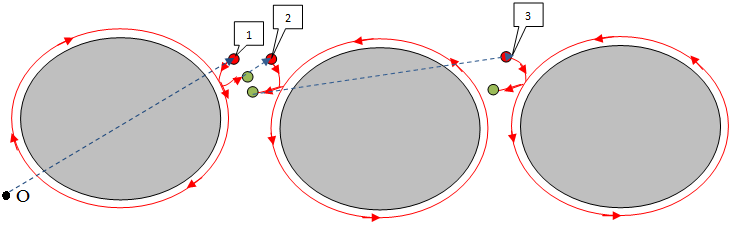
\includegraphics[width=0.9\textwidth]{3-3.png}
  \caption{Пример схемы резки трех круглых заготовок «по замкнутому» контуру}
  \label{3-3}
  \end{center}
\end{figure}

\begin{figure}
  \begin{center}
  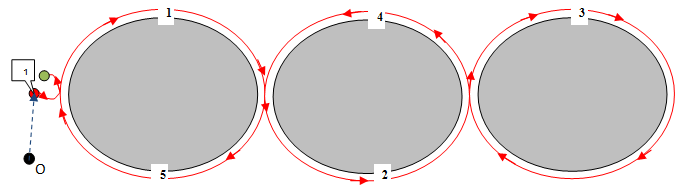
\includegraphics[width=0.9\textwidth]{3-1.png}
  \caption{Пример схемы резки трех круглых заготовок с применением специальной техники резки без дополнительного реза}
  \label{3-1}
  \end{center}
\end{figure}

На Рис. \ref{3-1}
цифрами от 1 до 5 показана последовательность
резки контуров за один сегмент,
т.е. после врезания в материал режущий инструмент
на рабочем ходе переходит к вырезке участка
под номером 1 первого контура,
затем без дополнительного реза режущая головка
переходит ко второму контуру и вырезает участок
контура под номером 2 и т.д.
В конце режущий инструмент завершает
вырезку трех контуров с одной точкой
врезки по пятому участку первого контура и
переходит к точке выключения.
Следует обратить внимание, что в рассматриваемом
способе резки инструмент переходит от одного контура к
другому на рабочем ходе без дополнительных резов,
за счет чего сокращаются значения основных параметров резки
$L_{on}, L_{off}, N_{pt}$.
Однако в результате применения предложенного метода
резки при обработке круглых заготовок в месте «стыковки»
контуров возможно образование «ступеньки»
(см. Рис. \ref{hiccup}),
что в некоторых случаях может привести к
искажению конечной геометрии и требуемых размеров заготовки.
Как показывает практика при обработке круглых заготовок на
машине лазерной листовой резки с ЧПУ размеры «ступеньки» незначительны
(достигают десятых-сотых долей мм)
и ее размеры либо попадают в требуемое поле допуска
для соответствующего размера, либо ее можно «зачистить»
с помощью дополнительной обработки без искажения геометрии и требуемых размеров.
Также следует отметить, что часто детали,
получаемые после лазерной обработки,
являются заготовками для дальнейших переделов с
припусками на требуемые размеры чертежа,
поэтому допускаются незначительные дефекты,
обработка которых в дальнейшем не приведет к
искажению требуемых размеров и форм конечной детали.

При размещении круглых заготовок в один ряд
либо вдоль оси Х, либо вдоль Y
возможно сокращение количества точек врезок до
$N_{pt}=1$
и сведение
$L_{off}$
к велечине, равной нулю, если не считать перемещения
режущего инструмента на холостом ходе до точки врезки
для текущего ряда круглых заготовок и от точки выключения
режущего инструмента до следующей точки врезки или нулевой точки
($L_{off} \approx 0$).
В случае размещения круглых заготовок в $n$
рядов при использовании предложенного способа резки
$N_{pt}=n$.

\begin{figure}
  \begin{center}
  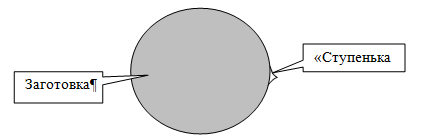
\includegraphics[width=0.7\textwidth]{hiccup.png}
  \caption{Возможная «ступенька» при обработке круглых заготовок с помощью специального метода резки}
  \label{hiccup}
  \end{center}
\end{figure}

Предложенный на рис. \ref{3-1}
метод резки круглых заготовок в основном применим для заготовок,
которые можно объединить в один блок и применить
данную специальную технику резки без дополнительного реза.
Однако на практике возникают случаи вырезки круглых заготовок
специальным способом с дополнительным резом
(рис. \ref{3-extra}).
Например, на производстве возникает задача
вырезки круглых заготовок разного габаритного размера,
также при построении маршрута перемещения режущего инструмента
на машинах термической резки с ЧПУ необходимо выполнение
технологических ограничений термической резки.
В частности, в случае необходимости выполнения условий
сокращения термических деформаций вырезку заготовок с
применением разработанной специальной техники резки
для круглых заготовок необходимо выполнять без изменения обхода контуров.
С этой целью может быть применим способ с дополнительным резом
(рис. \ref{3-extra})
во избежание повышения температуры в процессе резки контуров
в месте стыка деталей из-за острого угла
при переходе от одного контура к другому без изменения
направления обхода и во избежание образования «ступеньки».
Вырезка контуров осуществляется аналогично способу,
приведенному выше (рис. \ref{3-3}),
однако при переходе от одного контура к другому
при необходимости возможен дополнительный рез
(при наличии деталей значительно отличающихся по размерам и смещении друг относительно друга).
В свою очередь это может привести к увеличению
$L_{on}$
на величину фактической длины дополнительных резов
$L_\text{доп}^\text{факт}$.
Поэтому в данном способе необходимо вычислять максимально допустимую длину дополнительного реза
$L_\text{доп}$
и
$L_\text{доп}^\text{факт} \leqslant L_\text{доп}$.
На рис. \ref{3-extra}
красными стрелками показан спроектированный путь
перемещения инструмента на рабочем ходе при прямом обходе контуров,
фиолетовым – обратный ход режущего инструмента
при завершении вырезки трех деталей с
применением специальной техники резки.

\begin{figure}
  \begin{center}
  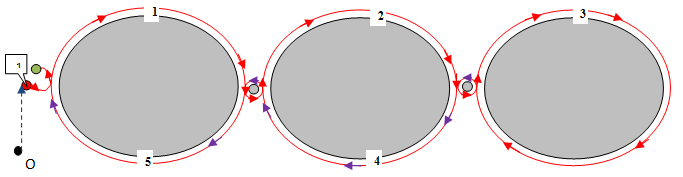
\includegraphics[width=0.9\textwidth]{3-extra.png}
  \caption{Пример схемы резки трех круглых заготовок с применением специальной техники резки с дополнительным резом}
  \label{3-extra}
  \end{center}
\end{figure}

Согласно предложенному методу режущая головка
после врезания в материал обходит по часовой
стрелки первый участок контура под номером 1,
после чего меняя направление обхода против
часовой стрелки совершает дополнительный рез и
переходит к вырезке участка под номером 2 второго
контура по часовой стрелке и т.д.
Пока режущий инструмент не завершит
вырезку полного контура с номером 3,
после чего режущая головка совершает обратный обход
оставшихся не вырезанных частей контуров под номерами 4 и 5.
Таким образом, можно вырезать заготовки разных размеров,
объединенных в блоки и внутри каждого блока реализовать
вырезку нескольких контуров с помощью одной точки врезки.
При этом дополнительный рез может быть выполнен по дуге,
либо по прямой в зависимости от размера внешнего контура заготовок.

С целью оценки эффективности в результате применения
разработанных специальных способов резки рассмотрим
пример резки круглых заготовок двумя вышеописанными
методами на машине лазерной листовой резки ByStar3015 с ЧПУ.
Для этого были разработаны две раскройные карты,
на которых были размещены 69 и 58 заготовок,
имеющих круглый наружный контур.

На рис. \ref{circles-a} и \ref{circles-b}
приведен маршрут резки
круглых заготовок одного размера без дополнительного реза,
на рис. \ref{circles-c} и \ref{circles-d} – с дополнительным резом.
Полученные результаты были сравнены с результатми
резки «по замкнутому контуру» и приведены в табл. 2.4.
Расчет был произведен для листового материала 12Х18Н10Т $\Delta$=1 и 5 мм.

\begin{figure}
  \begin{center}
  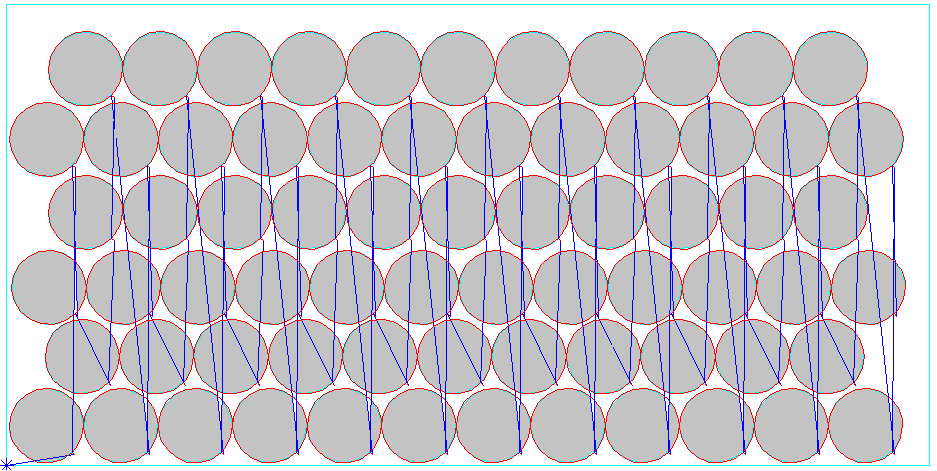
\includegraphics[width=0.9\textwidth]{circles-a.png}
  \caption{Пример маршрута резки круглых заготовок c применением резки «по замкнутому контуру»}
  \label{circles-a}
  \end{center}
\end{figure}

\begin{figure}
  \begin{center}
  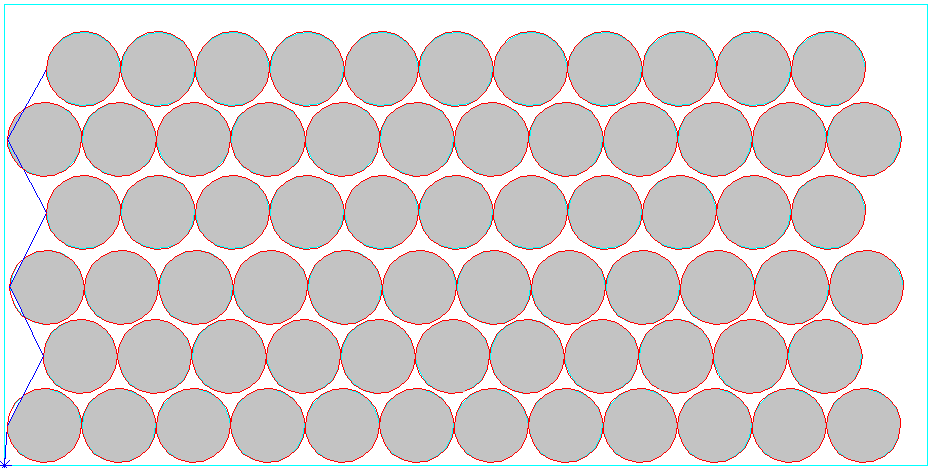
\includegraphics[width=0.9\textwidth]{circles-b.png}
  \caption{Пример маршрута резки круглых заготовок c применением метода резки без дополнительного реза}
  \label{circles-b}
  \end{center}
\end{figure}

На рис. \ref{circles-d}
разными цветами обозначены блоки деталей,
для которых реализована резка без дополнительного реза.
В частности, в нижней  части раскройной карты коричневым цветом
выделена группа из 10 круглых заготовок и одного кольца.
Размеры заготовок отличаются незначительно,
поэтому есть возможность реализовать резку блока из 11 деталей с
помощью одной точки врезки и без дополнительного реза.
В  верхней части той же раскройной карте выделен блок из шести деталей,
вырезаемых с одной точкой врезки, при этом заготовки,
выделенные фиолетовым цветом, вырезаются без дополнительного реза,
но при переходе к серым заготовкам меньшего размера необходимо
вырезку осуществить с дополнительным резом.
При этом дальнейшая вырезка трех серых заготовок
осуществляется без дополнительного реза.

\begin{figure}
  \begin{center}
  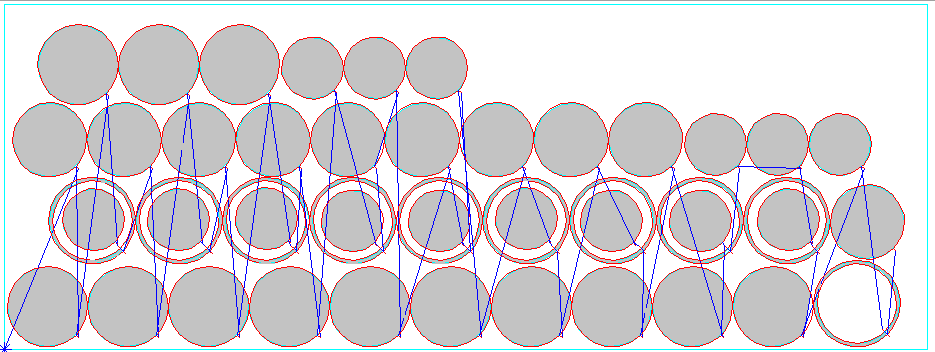
\includegraphics[width=0.9\textwidth]{circles-c.png}
  \caption{Пример маршрута резки круглых заготовок разного размера c применением резки «по замкнутому контуру»}
  \label{circles-c}
  \end{center}
\end{figure}

\begin{figure}
  \begin{center}
  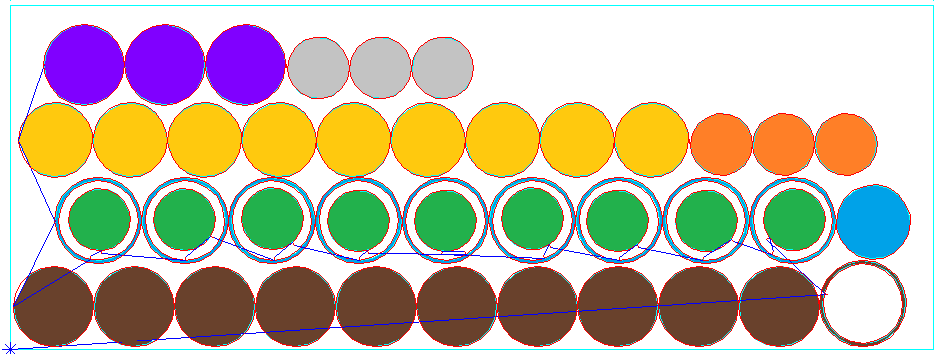
\includegraphics[width=0.9\textwidth]{circles-d.png}
  \caption{Пример маршрута резки круглых заготовок разного размера c применением специальной техники резки}
  \label{circles-d}
  \end{center}
\end{figure}

\begin{table}
  \begin{tabular}{cccccccccc}
    Марка & $\Delta$ & Резка & $L_{on}$, м & $L_{off}$, м & $N_{pt}$ & $F_{cost}$, руб & \% & $L_\text{доп}^\text{факт}$, м \\
    \hline
    \multirow{8}{*}{12Х18Н10Т} & \multirow{4}{*}{1 мм} & Стандартная & 54,7 &	43,07	& 69 & 1552,92 & \multirow{2}{*}{15,6} &	\multirow{2}{*}{-} \\
    & & Без доп. реза & 52,02 &	0,7 & 6 & 1310,05 \\
    & & Стандартная   & 46,14 & 18,78 & 58 & 1302,08 & \multirow{2}{*}{6,88} & \multirow{2}{*}{0,16} \\
    & & С доп. резом  & 46,3  & 5,43  & 23 & 1212,43 \\
    & \multirow{4}{*}{5 мм} & Стандартная & 54,7 &	43,07	& 69 & 12154,8 & \multirow{2}{*}{14,3} &	\multirow{2}{*}{-} \\
    & & Без доп. реза & 52,02 &	0,7 & 6 & 10417,2 \\
    & & Стандартная   & 46,14 & 18,78 & 58 & 10241,6 & \multirow{2}{*}{6,2} & \multirow{2}{*}{0,16} \\
    & & С доп. резом  & 46,3  & 5,43  & 23 & 9607,08 \\
  \end{tabular}
  \label{circles}
  \caption{Результаты расчета стоимость резки раскройного плана для круглых заготовок с применением специальных способов резки}
\end{table}

По результатам анализа приведенных в Табл. \ref{circles}
данных, можно сделать следующие выводы:

\begin{enumerate}
\item Применение специального метода резки круглых заготовок
без дополнительного реза (рис. \ref{circles-b})
приводит к сокращению количества точек врезок до 90\%
 и длины перемещений инструмента на холостом ходе до 98\%
 по сравнению с резкой по «замкнутому контуру».
 При проведении ряда экспериментов в среднем значение $N_{pt}$
 сокращается на 60\%, значение $L_{off}$ на – 65\%.
 При этом стоимость обработки раскройной карты в среднем сокращается на 15\%;

\item Применение резки с дополнительным резом (рис. \ref{circles-d})
приводит в среднем к сокращению количества точек врезок на 60\%,
а длины перемещений инструмента на холостом ходе сокращается на 70\%
по сравнению с резкой «по замкнутому контуру».
В свою очередь стоимость обработки сокращается на 7\%.
При этом следует отметить,
что по причине наличия внутренних контуров
наблюдается снижение эффективности применения
предложенных технологий;

\item В случае применения резки с дополнительным резом необходимо рассчитать
$L_\text{доп}^\text{факт}$.
и
$L_\text{доп}$
согласно (\ref{l-dop}) и (\ref{l-fact-dop}).
\end{enumerate}

\subsubsection{Стратегии проектирования маршрута режущего инструмента для многоугольных заготовок}

В машиностроительном производстве
при раскрое листового материала с помощью машин лазерной резки с ЧПУ
к наиболее часто встречающимся геометрическим
типам заготовок помимо круглых внешних контуров
относят также многоугольные заготовки,
часто выпуклые симметричные многоугольники с отверстиями различной формы.
В отдельную группу можно отнести треугольные и прямоугольные заготовки.
Следует отметить, что прямоугольные заготовки целесообразно обрабатывать
с помощью совмещенного реза.
Касательно остальных многоугольных (в т.ч. треугольных)
заготовок применение совмещенного реза не эффективно,
т.к. обычно с помощью одной точки врезки удается вырезать обычно две заготовки.
Также не эффективны другие специальные способы резки
(например, «цепная» резка или змейкой),
т.к. применение выделенных способов приводит к
сокращению количества точек врезок,
но
$L_{on}=const$
в лучшем случае или его увеличении,
что в свою очередь повышает время
$T_{cut}$
и стоимость раскроя
$F_{cost}$.
Поэтому возникает необходимость в разработке
новых специальных способов резки для выделенной группы заготовок.

В отдельную группу выделим треугольные заготовки,
для листовой резки которых на машине лазерной резки с ЧПУ
применим мультиконтурную резку,
совмещающую совмещенный рез и резку змейкой (рис.39).
На рис. \ref{6-6} приведена схема резки шести треугольных заготовок
одного размера с помощью резки «по замкнутому» контуру при этом
$N_{pt}=6$,
цифрами 1-6 обозначена последовательность резки.
На рис. \ref{6-1} приведена схема резки тех же шести
треугольных заготовок, при этом
$N_{pt}=1$.

\begin{figure}
  \begin{center}
  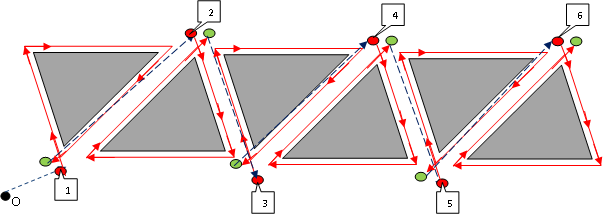
\includegraphics[width=0.9\textwidth]{6-6.png}
  \caption{Схема резки шести треугольных заготовок с помощью резки «по замкнутому контуру»}
  \label{6-6}
  \end{center}
\end{figure}

\begin{figure}
  \begin{center}
  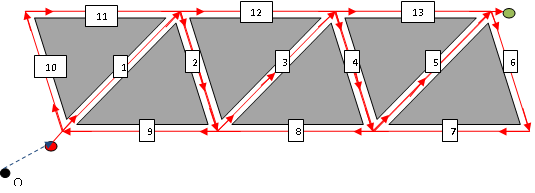
\includegraphics[width=0.9\textwidth]{6-1.png}
  \caption{Схема резки шести треугольных заготовок с помощью специального способа резки}
  \label{6-1}
  \end{center}
\end{figure}

Здесь цифрами 1-13 обозначена последовательность
резки контуров в одном сегменте,
т.е. после врезания в материал режущий инструмент
на рабочем ходе переходит к вырезке участка под номером 1
первого контура,
затем без дополнительного реза режущая головка
переходит ко второму контуру и вырезает участок под номером 2 и т.д.
В конце режущий инструмент завершает вырезку шести контуров
с одной точкой врезки по 13 участку и переходит к
точке выключения инструмента.
Следует обратить внимание, что в рассматриваемом способе
резки инструмент переходит от одного контура к другому
на рабочем ходе с совмещенным резом,
за счет чего сокращается количество точек врезок $N_{pt}$,
расстояние перемещений инструмента на рабочем $L_{on}$
и холостом  $L_{off}$ ходах.

Способ резки, предложенный на рис. \ref{6-1},
применим для групп треугольных заготовок одного типоразмера,
расположенных в два ряда.
При этом если количество рядов больше двух,
то создаются еще блоки заготовок,
каждый из которых включает в себя по 2 ряда треугольных заготовок.
Переход режущего инструмента от одного блока к другому
осуществляется с помощью холостого хода.
Внутри каждого блока реализована резка заготовок с одной точкой врезки.

В случае раскроя листового материала треугольными
заготовками можно спроектировать маршрут режущего
инструмента без холостого хода,
для этого треугольные заготовки необходимо
размещать согласно рис. \ref{3-10}.
Основное условие непрерывной резки нескольких
заготовок заключается в том,
что общее количество пересекающихся ребер у
любой вершины треугольника должно быть четным.
Или с точки зрения теории графов у каждой вершины
должно быть четное количество ребер.
В обратном случае непрерывную резку заготовок
с помощью одной точки врезки не осуществить
без дополнительных резов.
Например, как видно из рис. \ref{3-10}
общее количество обозначенных цифрами 1,2,4,5,7 и 8 ребер равно 6.

Цифрами 1-18 обозначена последовательность
резки контуров за один сегмент,
т.е. после врезания в материал режущий инструмент
на рабочем ходе переходит к вырезке участка
под номером 1 первого контура,
затем без дополнительного реза режущая
головка переходит ко второму контуру и
вырезает участок под номером 2 и т.д.
В конце режущий инструмент завершает
вырезку девяти контуров с одной точкой врезки
по 18 участку и переходит к точке выключения инструмента.
Следует обратить внимание, что в рассматриваемом способе
резки инструмент переходит от одного контура к
другому на рабочем ходе с совмещенным резом,
за счет чего сокращается количество точек врезок $N_{pt}$,
расстояние перемещений инструмента на рабочем ходе  $L_{on}$,
при этом
$L_{off} \approx 0$.
Холостой переход осуществляется
только при переходе режущего инструмента
от нулевой точки до точки врезки и от
точки выключения инструмента до нулевой точки.
Способом, приведенным на рис. \ref{3-10},
можно размещать большое количество
треугольных заготовок, при этом всегда $N_{pt}=1$
и $L_{off} \approx 0$.

\begin{figure}
  \begin{center}
  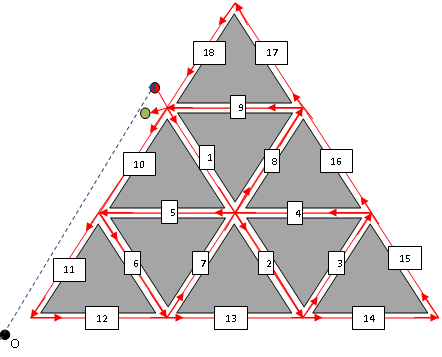
\includegraphics[width=0.8\textwidth]{3-10.png}
  \caption{Схема резки девяти треугольных заготовок с помощью мультиконтурной резки}
  \label{3-10}
  \end{center}
\end{figure}

Предложенные выше методы резки  применимы для любых треугольников.

Обработку пятиугольных заготовок из листового материала
на машине лазерной резки с ЧПУ также можно осуществить
предложенным методом, приведенным на рис. \ref{6-1}
с помощью мультиконтурной резки,
объединяющей совмещенный рез и резку змейкой.
На рис. \ref{5-6}
приведена схема резки «по замкнутому» контуру
шести пятиугольных заготовок при этом $N_{pt}=6$.

\begin{figure}
  \begin{center}
  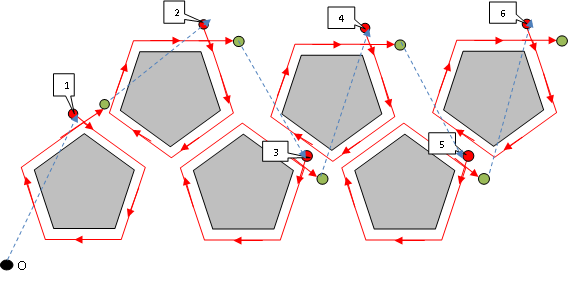
\includegraphics[width=0.9\textwidth]{5-6.png}
  \caption{Схема резки «по замкнутому контуру» шести пятиугольных заготовок}
  \label{5-6}
  \end{center}
\end{figure}

На рис.\ref{5-1}
предложена схема резки тех же шести
пятиугольных заготовок за один сегмент, при этом  $N_{pt}=1$
и $L_{off} \approx 0$.

\begin{figure}
  \begin{center}
  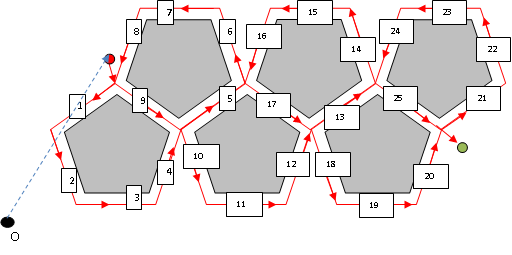
\includegraphics[width=0.9\textwidth]{5-1.png}
  \caption{Схема резки шести пятиугольных заготовок с мультиконтурной резки}
  \label{5-1}
  \end{center}
\end{figure}

С помощью схемы, приведенной на рис. \ref{5-1},
можно осуществлять резку по ребрам многоугольников,
соблюдая последовательность и направление резки каждого ребра.
Инструмент перемещается на холостом ходе от
начальной точки положения инструмента
(точки .О)
до точки врезки, после чего осуществляется непрерывная резка всех ребер,
начиная с 1, без дополнительных резов за один сегмент.
После того как режущий инструмент частично вырежет
первый контур по 4 ребрам (с 1 по 4)
переходит к 5 ребру и начинает вырезать
второй контур последовательно вырезая с 6 по 9 ребра.
При вырезке 9 ребра будут окончательно
вырезаны первый и второй контура.
Аналогично можно вырезать оставшиеся контура,
после чего инструмент переходит в точку выключения инструмента.
Как видно из рис. \ref{5-1},
за счет применения совмещенного реза сокращается $L_{on}$,
за счет отсутствия холостых переходов
$L_{off} \approx 0$
и $N_{pt}=1$
при одновременном сокращении общего времени
и стоимости резки заготовок из листового
материала на машинах лазерной резки с ЧПУ.
Предложенный способ резки применим для любых выпуклых пятиугольников.

В случае обработки четырехугольных заготовок
целесообразно применять совмещенный рез,
либо технологию, предложенную на рис. \ref{5-1},
при условии, что общее количество ребер,
пересекающихся в любой внутренней вершине, будет четным.
В последнем случае по сравнению с совмещенным резом значения
$N_{pt}$
и $L_{off}$
при использовании разработанного способа резки будут,
как правило, ниже, чем при совмещенном резе.
Но данный способ резки не всегда применим
с точки зрения снижения КИМ.

В общем случае при резке любых многоугольных
заготовок для случая,
когда количество пересекающихся ребер у вершин
(в частности внутренних) нечетно,
то предложенный способ резки реализуем с
дополнительным резом, либо с добавлением точек врезок.
Следует обратить внимание на то,
что при мультиконтурной резке многоугольников с
дополнительным резом, значение
$L_\text{доп}^\text{факт}$.
также как и для треугольников должно удовлетворять условию
$L_\text{доп}^\text{факт} \leqslant L_\text{доп}$,
рассчитанному по (\ref{l-fact-dop}),
в иначе значения целевых функций (\ref{cutting-time})
и (\ref{cutting-cost})
окажутся больше значений,
получаемых  при резке «по замкнутому контуру».
На рис. \ref{5-extra}
для любой вершины количество пересекающихся ребер нечетно,
поэтому резка контуров возможна только с дополнительным резом.
Цифрами 1-19 обозначена последовательность обхода ребер
пяти заготовок.
Режущий инструмент на холостом ходе переходит
из начальной точки в точку врезки,
после чего по эквидистантому контуру
осуществляется частичная вырезка первого
контура по ребрам 1-4,
затем вырезается ребро 5 второй заготовки и т.д.
пока окончательно не будут вырезаны пять заготовок по ребрам 6-19.
По причине наличия дополнительных резов рабочая
длина перемещения режущего инструмента может увеличиться по сравнению с $L_{on}$,
полученной в результате применения резки «по замкнутому контуру»,
поэтому актуален вопрос расчета
$L_\text{доп}^\text{факт} \leqslant L_\text{доп}$.
В результате применения предложенного на рис. \ref{5-extra}
специального метода резки
$N_{pt}=1$
и $L_{off} \approx 0$.

\begin{figure}
  \begin{center}
  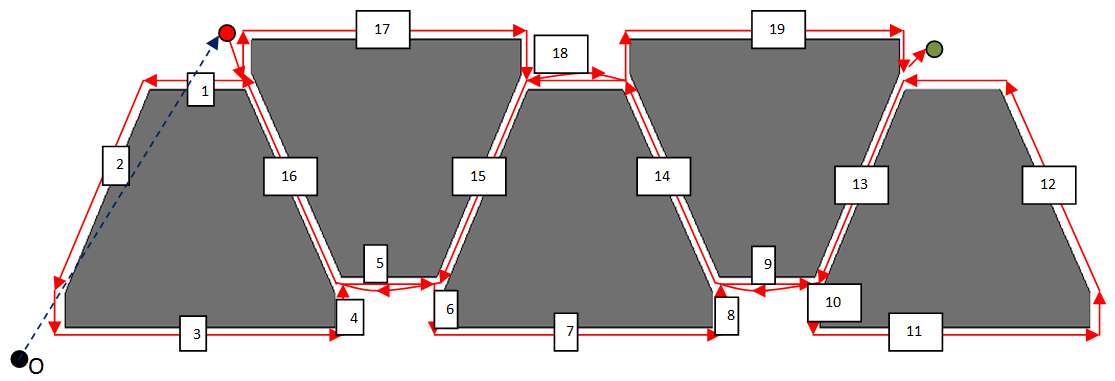
\includegraphics[width=0.9\textwidth]{5-extra.png}
  \caption{Схема резки пяти заготовок с помощью мультиконтурной резки с дополнительным резом}
  \label{5-extra}
  \end{center}
\end{figure}

Рассмотрим пример раскроя листового материала
12Х18Н10Т ($\Delta$=1-8мм)
многоугольными заготовками на машине лазерной резки с ЧПУ.
Для этого разработаны две раскройные карты с одинаковым количеством,
видом и размерами деталей,
для которых спроектирован маршрут перемещения
режущего инструмента в САПР «СИРИУС» с
применением резки «по замкнутому контуру» (рис. \ref{multi-a})
и специальной техники резки для многоугольных заготовок (рис.45).
Полученные результаты, которые содержат значения
$L_{on}$, $N_{pt}$, $L_{off}$, $T_{cut}$ и $F_{cost}$
для каждой раскройной карты, приведены в Таблице 5.

\begin{figure}
  \begin{center}
  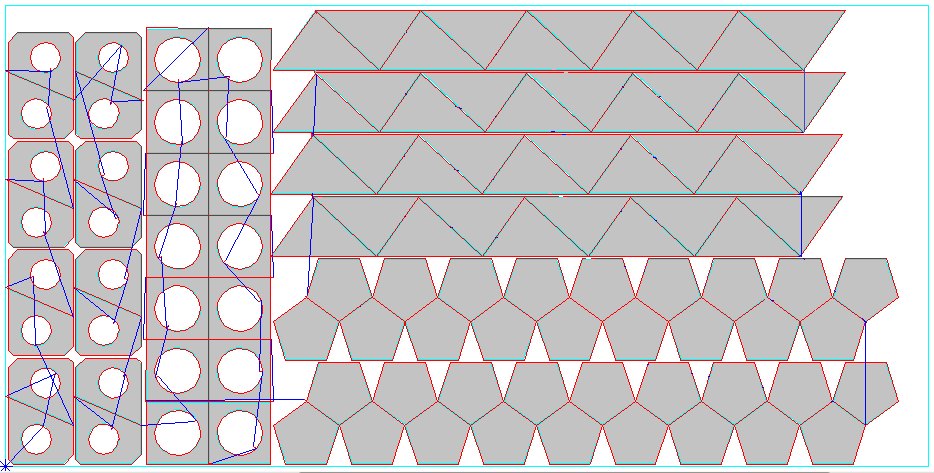
\includegraphics[width=0.9\textwidth]{multi-a.png}
  \caption{Схема раскройной карты с применением мультиконтурной резки для многоугольных заготовок}
  \label{multi-a}
  \end{center}
\end{figure}

\begin{figure}
  \begin{center}
  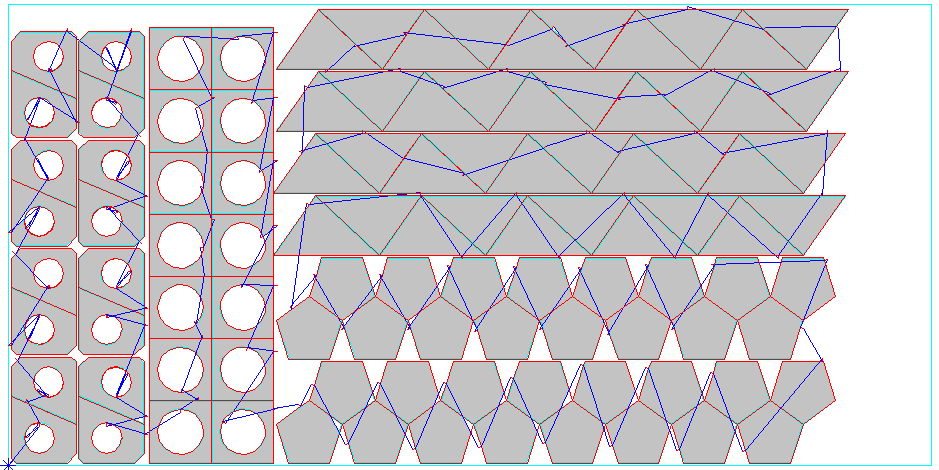
\includegraphics[width=0.9\textwidth]{multi-b.png}
  \caption{Схема раскройной карты с применением резки «по замкнутому контуру»}
  \label{multi-b}
  \end{center}
\end{figure}

Применение предложенных специальных методов резки
приводит к значительному сокращению значений
$N_{pt}$, $L_{on}$ и $L_{off}$
в сравнении со стандартной техникой резки
соответственно до 70\%, 27\% и 67\%
при одновременном сокращении времени
$T_{cut}$
и стоимости лазерной резки
$F_{cost}$ до 36\%.
Как показывает практика применения
предложенных методов резки при проектировании
УП в реальном производственном процессе,
в среднем значения параметров
$L_{on}$, $N_{pt}$  и $L_{off}$
сокращаются на 3\%, 60\% и 65\%
соответственно при одновременном снижении
$F_{cost}$
на 10-20\%
по сравнению с резкой «по замкнутому контуру».
Как видно из табл. \ref{polygons},
с увеличением толщины обрабатываемого материала
сокращается эффективность предложенных специальных способов резки.

\begin{table}
  \begin{tabular}{cccccccc}
    Марка & $\Delta$ & Резка & $L_{on}$, м & $L_{off}$, м & $N_{pt}$ & $F_{cost}$, руб & \% \\
    \hline
    \multirow{2}{*}{12Х18Н10Т} & \multirow{2}{*}{1 мм} & Стандартная & 101,85 & 26,92 & 163 & 2956,14 & \multirow{2}{*}{36} \\
    & & Специальная & 74,73 & 8,9 & 51 & 1901,4 \\
    \multirow{2}{*}{12Х18Н10Т} & \multirow{2}{*}{3 мм} & Стандартная & 101,85 &	26,92 & 163 & 9170,09 & \multirow{2}{*}{36.5} \\
    & & Специальная & 74,73 & 8,9 & 51 & 5823,10 \\
    \multirow{2}{*}{12Х18Н10Т} & \multirow{2}{*}{5 мм} & Стандартная & 101,85 & 26,92 & 163 & 23262,44 & \multirow{2}{*}{32.2} \\
    & & Специальная & 74,73 & 8,9 & 51 & 15768,17 \\
    \multirow{2}{*}{12Х18Н10Т} & \multirow{2}{*}{8 мм} & Стандартная & 101,85 & 26,92 & 163 & 94070,86 & \multirow{2}{*}{29.7} \\
    & & Специальная & 74,73 & 8,9 & 51 & 66121,93 \\
  \end{tabular}
  \label{polygons}
  \caption{Результаты расчета стоимости резки раскройного плана для многоугольных заготовок}
\end{table}

Выводы:

\begin{enumerate}
\item Применение специальных методов резки
для различных многоугольных заготовок возможно
без дополнительных резов между заготовками при условии,
что количество пересекающихся ребер у вершин
(в частности внутренних) четно.
В остальных случаях резка разработанным
способом резки возможна с дополнительным резом,
либо с увеличением числа точек врезок.
Предложенные методы базируются на известных методах резки
(змейкой и совмещенный рез),
за счет этого значительно сокращаются
значения основных параметры
$L_{on}$, $N_{pt}$  и $L_{off}$
и   при одновременном снижении
$T_{cut}$
и
$F_{cost}$;

\item В зависимости от типа заготовок,
наличия или отсутствия отверстий в деталях
количество точек врезок может снизиться до
$N_{pt}=1$,
при этом
$L_{off} \approx 0$.
В рассмотренных примерах значения
$N_{pt}$, $L_{off}$ и $L_{on}$
иаксимально сокращаются соответственно до 70\%, 67\% и до 27\%
при одновременном сокращении
$T_{cut}$
и
$F_{cost}$
до 36\%.
В среднем значение $F_{cost}$ снижается на 10-20\%;

\item При применении предложенных специального способа резки
для многоугольных деталей с дополнительным резом
необходимо вычислять значение
$L_\text{доп}^\text{факт}$:
$L_\text{доп}^\text{факт} \leqslant L_\text{доп}$.
В противном случае значение
$L_\text{доп}$.
может оказаться больше значения
$L_{on}$,
полученное при резке «по замкнутому контуру»,
что в свою очередь может привести к увеличению значений целевых функций
$T_{cut}$
и
$F_{cost}$.

\item Эффективность от применения предложенных способов резки
сокращается при увеличении толщины обрабатываемого материала.
\end{enumerate}

{\bf Заключительные замечания}

Предложенные способы применения специальных техник резки и
формирование групп однотипных заготовок на этапе
проектирования раскроя листовых материалов на фигурные заготовки,
среди которых присутствуют круглые и многоугольные,
можно интерпретировать как методы формирования наборов базовых сегментов
(а в дискретном случае – мегаполисов)
для последующего решения задач оптимизации класса GSCCP
средней и большой размерности.
Это создаёт, в свою очередь,
предпосылки  для разработки эффективных методов
решения интегрированной задачи раскроя и мсаршрутизации,
для которой целевая функция стоимости складывается
из стоимости использованного материала для раскроя
и стомости процесса резки
$
F_{cost}=
L_{on} \cdot C_{on} +
L_{off} \cdot C_{off} +
N_{pt} \cdot C_{pt}
$.

\subsection{Разработка методов учёта динамических ограничений
  в оптимизационных алгоритмах маршрутизации инструмента машин для термической резки листовых зашотовок}

Как отмечалось в параграе 1.3.
%%% TODO fix reference ^^^^^^^^^^^^^
наиболее сложной проблемой при разработке методов оптимизации
траектории инструмента машин листовой резки с ЧПУ
является математическая формализация и
разработка вычислительных алгоритмов учета
технологических эвристических требований термической резки,
т.н. правил «жёсткости детали»и «жёсткости листа».
«Динамический» характер этих условий, заключающийся в том,
что сами ограничения формируются только в процессе вычисления
допустимого решения задачи, по сути порождает
новый не исследованный ранее класс маршрутных задач
с крайне сложными видами ограничений типа (1.3.5).

Ниже приведен способ формализациии правила «жёсткости детали»,
основанный на введении понятия «зона жесткости».

{\it Определение 5}.
Зоной жесткости называется область,
ограниченная следующими четырьмя геометрическими кривыми:
1)траекторией инструмента;
2)эквидистантной этой траектории кривой, отстоящей на величину $R$;
3)прямой, проходящей через точку выключения инструмента $M^*$
перпендикулярно траектории инструмента в этой точке;
4) прямой, проходящей через точку,
отстоящую от точки выключения инструмента $M^*$ на некоторую величину $L$,
перпендикулярно траектории инструмента в этой точке.

Параметры этой зоны для двух точек
(длина $L$ и радиус $R$)
определяются в каждом конкретном случае
на основании эксперной оценки,
зависящей, в частности, от марки и толщины материала,
а также технологии термической резки.
На Рис. \ref{hardness-area}
эти зоны выделены жёлтым цветом.

\begin{figure}
  \begin{center}
  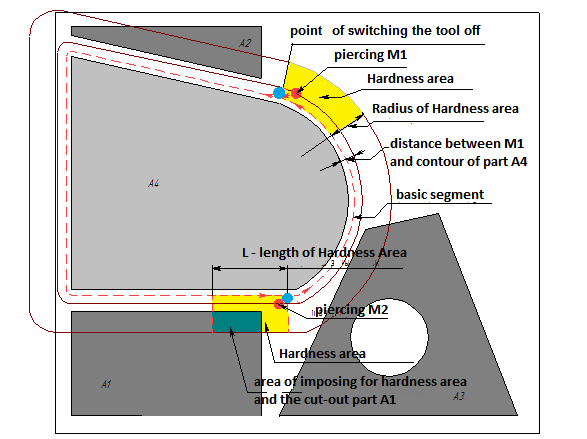
\includegraphics[width=0.9\textwidth]{hardness-area.png}
  \caption{Формализация правила «жёсткости детали» на основе понятия «зоны жёсткости»}
  \label{hardness-area}
  \end{center}
\end{figure}

Тогда в оптимизационных процедурах машрутизации
для задачи GTSP  и дискретных моделей задач CCP, SCCP, GSCCP
выбор точки врезки M и точки выключения инструмента $M^*$
(сегмента резки) определяется простым условием:
{\bf Зона жёсткости} должна лежать в ещё невырезанной
«жёсткой» части листового материала.
Для тех точек врезки, для которых это условие не выполнено,
значение целевых функций  увеличивается на некоторую величину «штрафа».

Как нетрудно видеть,
сформулированное правило выбора «хороших» точек врезки
и точек выключения инструмента носит геометрический характер.
Поскольку технологическое правило «жёсткости» детали
связано с тепловыми деформациями материала,
то естественно предположить,
что температура в «хороших» зонах«жёсткости будет меньше,
чем в «плохих».
В случае справедливости этой гипотезы,
адекватная оценка тепловых деформаций материала
при термической резке заготовок на машинах с ЧПУ
может иметь важное значение как инструмент
обеспечения необходимых технологических требований.
Для проверки гипотезы необходимо иметь инструментарий
моделирование и вычисления тепмерратуры тепловых полей в
каждый момент времени процесса резки.
Для разработки необходимого программного
обеспечения рассмотрим следующую задачу.

{\bf Постановка задачи}

Имеется металлическая пластина.
Заданы контуры, последовательность их резки,
точки врезки и направления обходов.
Для режущего инструмента заданы «радиус теплового луча»,
мощность, скорость перемещения и скорость холостого хода.
Требуется рассчитать тепловые поля при
последовательной резке контуров.

{\bf Расчет процесса резки контуров}

Последовательно для каждого контура рассматривается задача нахождения
$\theta(t, x)$ - температуры
($t$ -момент времени,
$x$ - точка области), удовлетворяющей уравнению теплопроводности
\begin{equation}
c \rho \frac{\partial \theta}{\partial t}=k \Delta \theta +N, x \in \Omega
\end{equation}
начальному условию
\begin{equation}
  \theta(t_0, x)=\theta_0(x), x \in \Omega
\end{equation}
граничному условию
\begin{equation}
  -k \frac{\partial \theta}{\partial n}=M(\theta - \theta_*), x \in \partial \Omega
\end{equation}
$t$ из промежутка $[t_0, t_1]$,
$x$ - точка области
$\Omega \subset \mathbb R^3$.

Здесь
$t_0$ - время начала и
$t_1$  - время окончания резки текущего контура,
$\Omega$ - часть пластины, которая осталась после удаления областей,
ограниченных предыдущими контурами,
$\partial \Omega$ - граница области $\Omega$.
$c$ – удельная массовая теплоемкость,
$\rho$ – плотность,
$k$ – коэффициент теплопроводности,
$N(t,x)$ – плотность тепловых источников,
$M$ - коэффициент теплопередачи,
$\theta_0(x)$ - текущее температурное поле перед началом резки данного контура,
$\theta_*$ -температура воздуха.

Функция $N$ - плотность тепловых источников имеет следующий вид.
Пусть толщина листа  $h$,
«радиус теплового луча» $r$,
его мощность w и скорость перемещения $v$.
Пусть  $m(t)$ – положение оси теплового «луча» в момент $t$.
Тогда
$p=w/(\pi r^2 h)$
плотность мощности теплового «луча» и
$N(t,x)=p$
в точках, находящихся от прямой $m(t)$
на расстоянии меньше $r$  и
$0$ в остальных точках.

{\bf Аппроксимация задачи}

Процесс пересчета температурного поля
$\theta(t, x)$
во время резки контура
разбивается на малые промежутки времени
$[t_{r-1}, t_r]$
длины  $\Delta t$
и для расчета
$\theta(x)=\theta(t_r, x)$
рассматривается задача

\begin{equation}
c \rho \frac{\theta(x)-\theta_0(x)}{\Delta t}=k \Delta \theta(x) + N(X)
\end{equation}
\begin{equation}
  -k \frac{\partial \theta}{\partial n}=M(\theta - \theta_*)
\end{equation}
где
$\theta_0=\theta(t_{r-1}, x)$
и
$N(x)=N(t_{r-1},x)$.

Область
$\Omega$
разбивается на тетраэдры,
функции
$\theta(x), \theta_0(x), N(x)$ - кусочно-линейные,
определяемые значениями в узлах – вершинах тетраэдров.
Решение данной задачи является точкой минимума следующего функционала

\begin{multline}
  I(\theta) =
  \frac{1}{2 \Delta t} \int\displaylimits_\Omega c \rho (\theta - \theta_0)^2 dx
  + \frac12 \int\displaylimits_\Omega k |\nabla \theta|^2 dx \\
  - \int\displaylimits_\Omega N \theta dx
  + \frac12 \int\displaylimits_{\partial \Omega} M(\theta - \theta_*)^2 dS
\end{multline}

Нахождение точки минимума данного квадратичного фунционала
проводится методом релаксации.
Выбор метода основан на следующих соображениях.

Так как радиус  $r$
«теплового луча» мал,
то тетраэдры разбиения области должны иметь малый размер
(в расчетах длина сторона была  2 мм)
и поэтому их много.
В узлах, далеких от точек где уже был «тепловой луч»
и куда еще не могло дойти изменение тепла к данному моменту времени,
температура остается первоначальной.
Метод релаксации позволяет пропустить такие узлы,
что позволяет уменьшить время счета.

{\bf Замечание}.
Для уменьшения числа тетраэдров (узлов)
при расчете резки очередного контура
$K_i$
рассматривается не вся оставшаяся пластина, а кусок
$\Omega_i \supset \Omega_{i-1}$.
Кусок  достаточно большой,
чтобы к моменту завершения резки контура
$K_i$
температура вне
$\Omega_i$
не могла измениться.
После завершения резки контура
тетраэдры внутри контура удаляются и их число уменьшается.
Дальше производится расширение СКЭ до следующего куска
$\Omega_{i+1}$.

{\bf Просмотр результатов}

Разработанное программное обеспечени
позволяет просматривать изменение температурных полей
в процессе резки.
На рис. \ref{thermal-plan}
показан пример задания порядка резки
6-ти заготовок (8 контуров),
точек врезки и направление обхода
(минус означает обход по часовой стрелке).
Материал пластины -  сталь 12Х2Н4А,
толщина $h$ = 2 мм, размеры 1000 $\times$ 1000 мм.
Радиус «теплового луча» $r$ = 2 мм,
мощность $w$ = 1000 вт,
скорость $v$ = 10 м/с.

На рис. \ref{thermal-5} показано температурное поле
на одной из стадий процесса резки 5-го контура.

{\bf Замечание}.
Рисунки \ref{thrm-high} и \ref{thrm-low}  иллюстрирую справедливость гипотезы.
Эти процессы отличаются только выбором точкой врезки.
На рис. \ref{thermal-high} точка врезки вблизи кромки пластины.
Средняя температура в выделенном окне
вокруг точки завершения резки контура 480$^o$С.
На рис. \ref{thermal-low} точка врезки далеко от кромки.
Средняя температура в выделенном окне  362$^o$С.

\begin{figure}
  \centering
  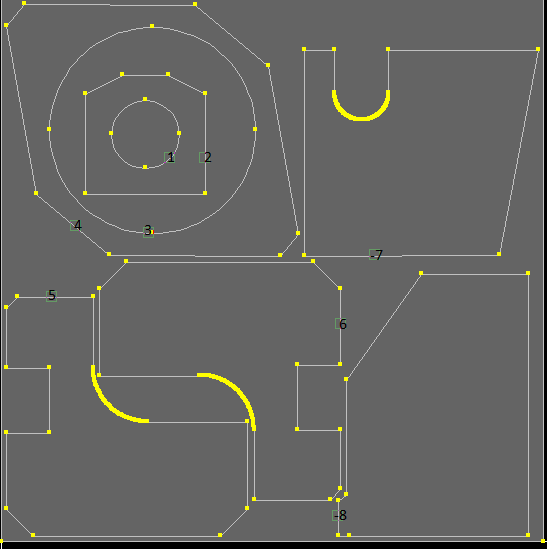
\includegraphics[width=0.6\textwidth]{thermal-plan.png}
  \caption{Места точек врезки и порядок резки для 8-ми контуров}
  \label{thermal-plan}
\end{figure}

\begin{figure}
  \centering
  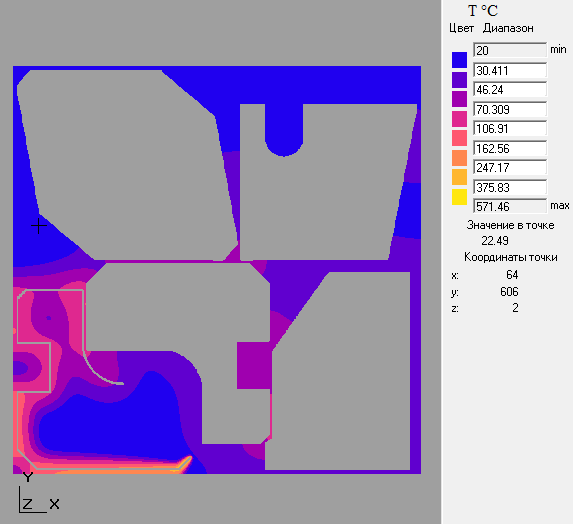
\includegraphics[width=0.7\textwidth]{thermal-5.png}
  \caption{Пример распределения тепловых полей в процессе резки 5-го контура}
  \label{thermal-5}
\end{figure}

\begin{figure}
  \centering
  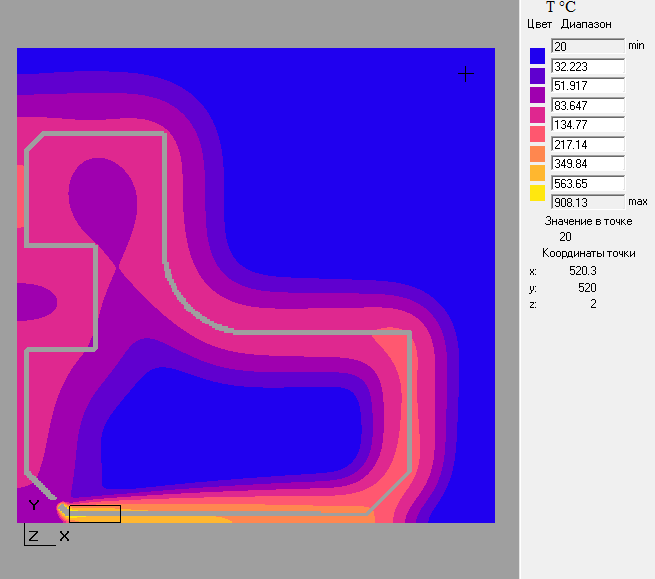
\includegraphics[width=0.6\textwidth]{thermal-high.png}
  \caption{Температурное поле при выборе точки врезки вблизи края пластины}
  \label{thrm-high}
\end{figure}

\begin{figure}
  \centering
  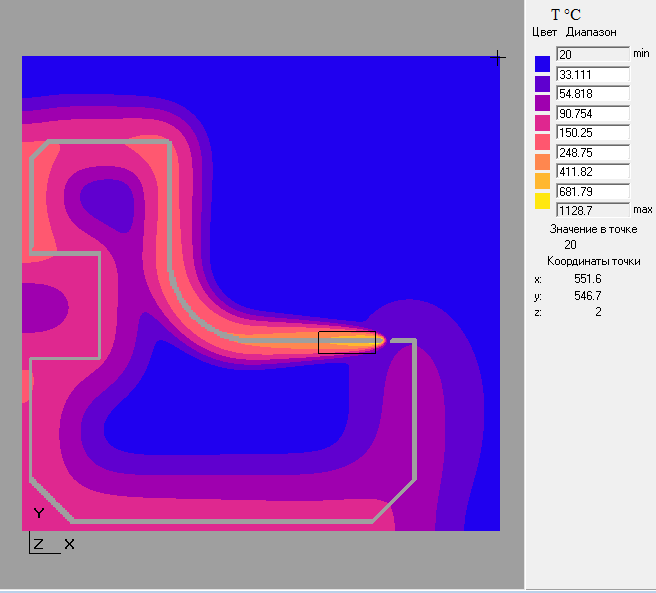
\includegraphics[width=0.6\textwidth]{thermal-low.png}
  \caption{Температурное поле при выборе точки врезки вдали от края пластины и границ вырезанных заготовок}
  \label{thrm-low}
\end{figure}

Другие проведенные вычислительные эксперименты
также показали уменьшение температуры материала
в «хороших» зонах в среднем на 63\%.
Ниже приведены ещё два примера расчета температурных полей.

\begin{figure}
  \centering
  \subfigure[309 градусов Цельсия (точка выключения инструмента не удовлетворят правилу «жесткости детали») ]{
    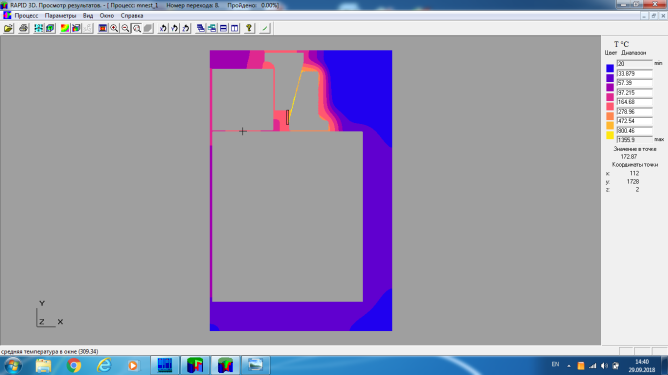
\includegraphics[width=0.9\textwidth]{thermal-309.png}
    \label{thermal-309}
  }
  \subfigure[120 градусов (точка выключения удовлетворят данному правилу)]{
    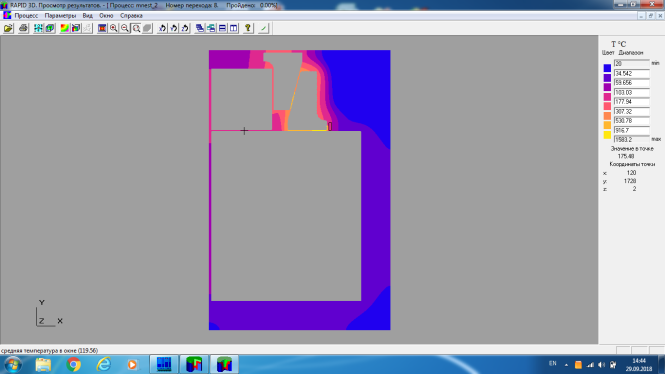
\includegraphics[width=0.9\textwidth]{thermal-120.png}
    \label{thermal-120}
  }
  \caption{Уменьшение температуры металла в зоне жёсткости }
  \label{thermal-309-120}
\end{figure}

Таким образом,
анализ температурных полей подтверждает
геометрические правила выбора точек врезки
и точек выключения инструмента машин термической
резки материала и в будущем
(при условии разработки быстродействующих систем температурного анализа)
может сам служить средством для выбора точек начала и конца сегментов резки.

\begin{figure}
  \centering
  \subfigure[550 градусов]{
    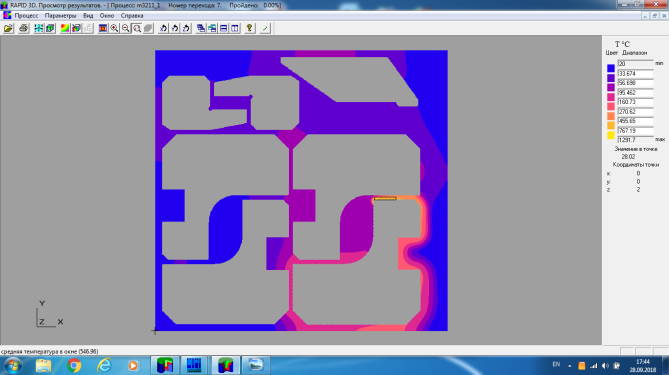
\includegraphics[width=0.9\textwidth]{thermal-550.png}
    \label{thermal-550}
  }
  \subfigure[130 градусов]{
    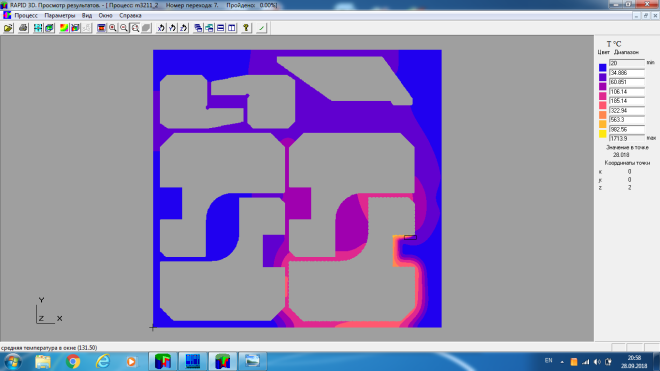
\includegraphics[width=0.9\textwidth]{thermal-130.png}
    \label{thermal-130}
  }
  \caption{Уменьшение температуры металла в зоне жёсткости }
  \label{thermal-550-130}
\end{figure}



Рассмотрим далее один из простых способ учета правила жесткости листа,
описанного в параграфе 1.3,
основанный на делении области листа на
последовательный набор подобластей (зон) (1.3.3):
$$
B_j =
\bigcup_{r=1}^l \Omega_r
$$

Способ заключается в том,
что после определения направления вырезки деталей на листе
(например, слева направо),
область листа разбивается вертикальными линиями
на прямоугольники одинакового размера.
Количество прямоугольников ($l$)
варьируется от 4 до 10 в зависимости от
геометрических размеров деталей
(чем крупнее размеры прямоугольников,
тем меньше формируется число зон).
Затем в каждой зоне решается основная задача (\ref{problem-statement})
уже без учета требований жёсткости листа,
но с учётом правила «жёсткости детали»
с помощью  алгоритма, описанного выше в этом параграфе.

На Рис.\ref{zones-a}
приведён пример оптимизации траектории
инструментадля задачи GTSP с учётом
формирования подобластей  (1.3.3).
Число подобластей в данном примере – 5.

\begin{figure}
  \begin{center}
  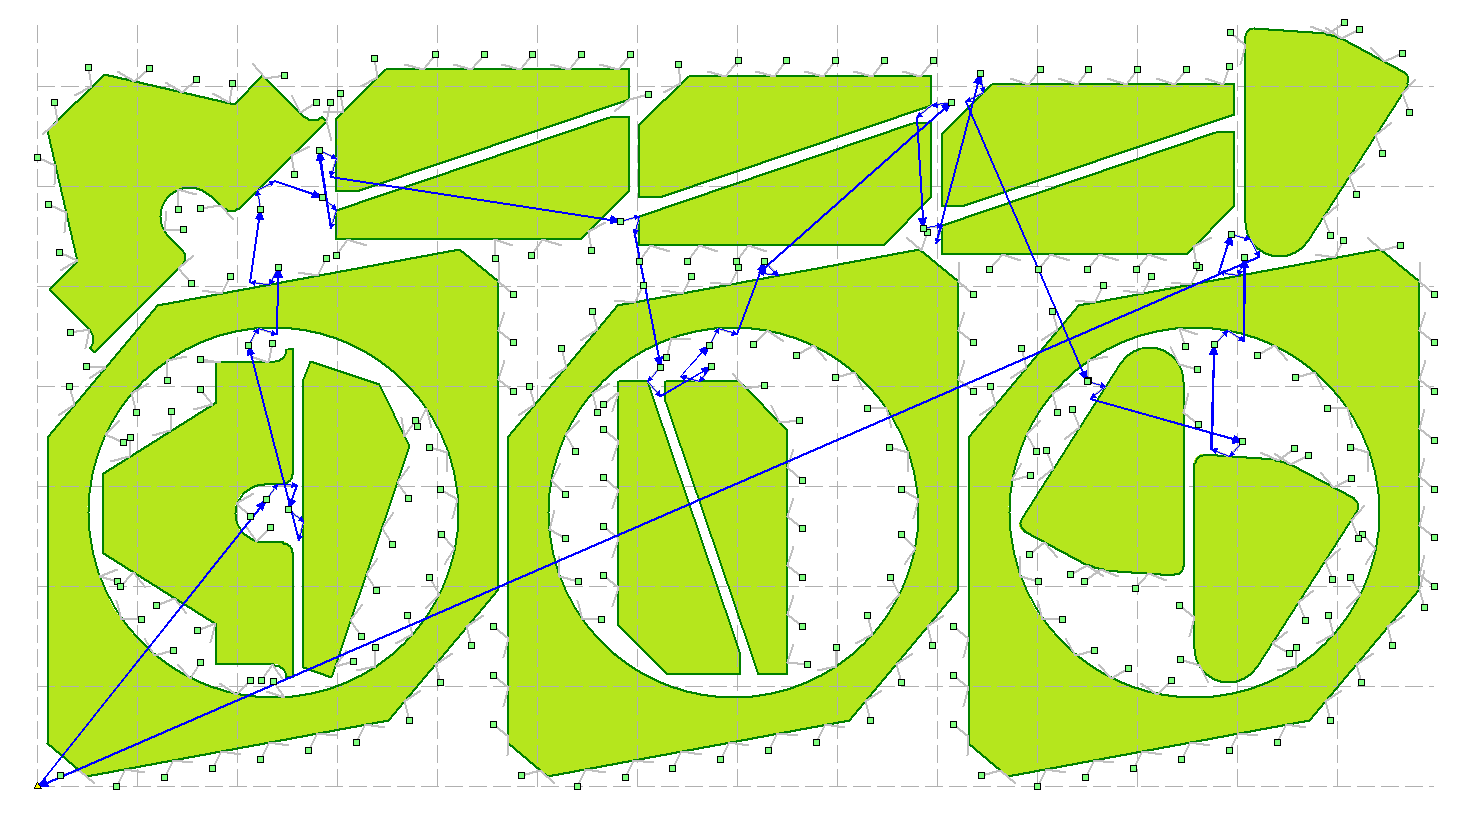
\includegraphics[width=0.9\textwidth]{zones-a.png}
  \caption{Пример моделирования траектории инструмента машины листовой резки с ЧПУ
    с учетом правила «жёсткости листа» и с использованием зон (20 контуров, задача GTSP)}
  \label{zones-a}
  \end{center}
\end{figure}

На Рис. \ref{zones-b}
эта же задача решена без учёта
«динамических» ограничений
(и правила жёсткости детали и правила жёсткости листа).
Ограничения на координаты точек врезки и
точки выключения инструмента,
обусловленные деформацией материала при врезке и
условия предшествования были соблюдены.
В качестве оптимизационного алгоритма
использован метод динамического программирования,
т.е. решение является глобальным экстремумом.
При этом для этого решения в маршруте резки
длина холостого хода инструмента уменьшилась на 26\%.

\begin{figure}
  \begin{center}
  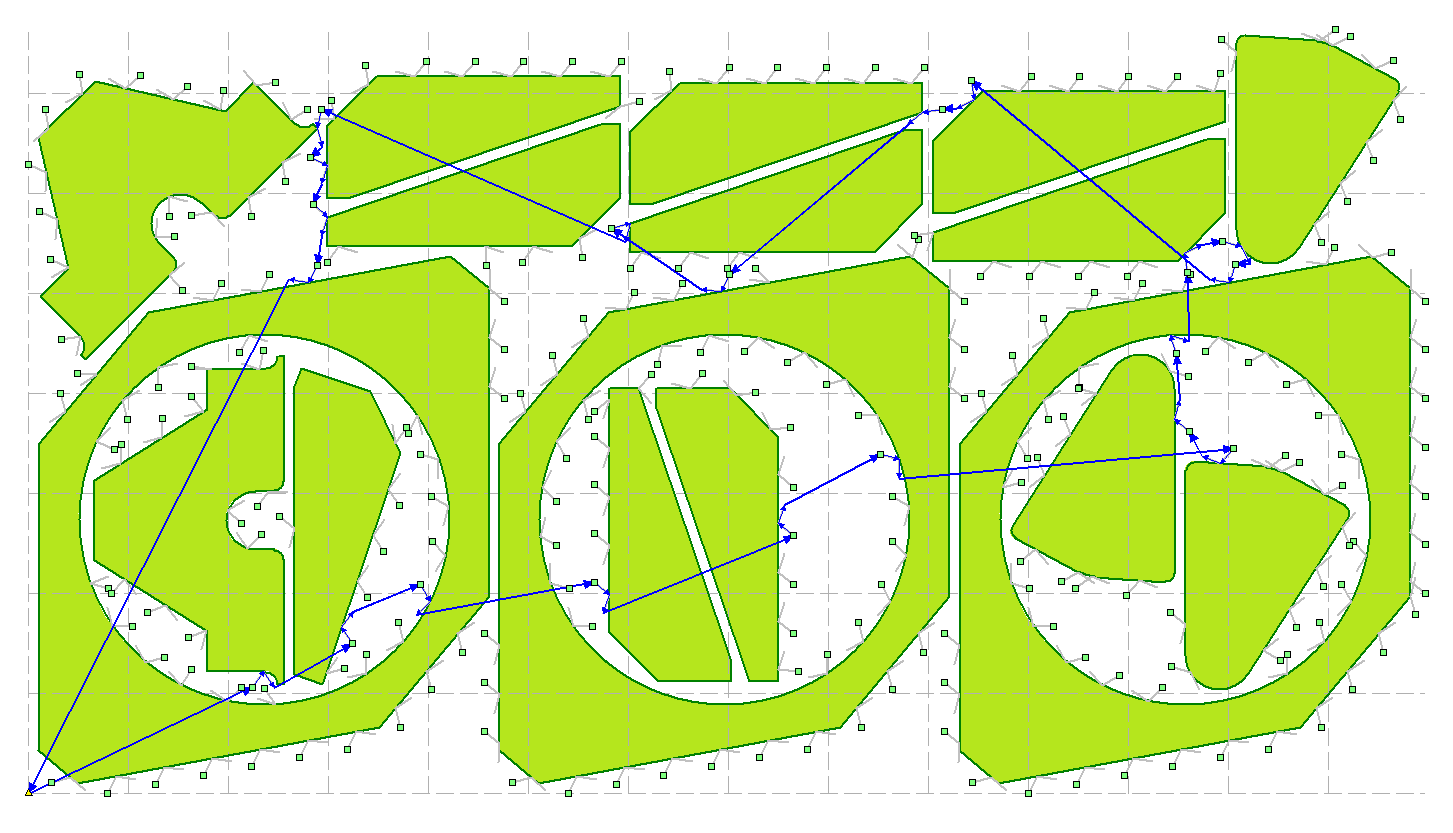
\includegraphics[width=0.9\textwidth]{zones-b.png}
  \caption{Схема оптимального маршрута резки для примера на Рис. \ref{zones-a}}
  \label{zones-b}
  \end{center}
\end{figure}


{\bf Заключительные замечания}

Описанные в данном параграфе практические методы учёта
правил жесткости детали и жёсткости листа позволяют
имплементировать их в существующие оптимизационные
алгоритмы решения задаяи (\ref{problem-statement})
с целевыми функциями \ref{cutting-time} - \ref{cutting-cost}
и получать рациональные варианты маршрута резки,
уменьшающие геометрические искажения деталей
при термической резке для большинства практических задач.
Вместе с тем, следует отметить,
что описанные способы в некоторых случаях не гарантируют 100\%
соблюдения технологических требований и
приводят к существенным тепловым деформациям материала.
Помимо этого остаётся открытым вопрос о разработке
эффективных алгоритмов получения глобальных экстремумов или
близких к ним для решения задач большой размерности с
одновременным учётом всех технологических требований
термической резки, включая динамические ограничения.
Этот вопрос  пока ещё ждёт своего решения.

\end{document}
